\title{\textbf{Infini-Attention: Compressive Memory with Sliding-Window Local Attention for Transformer Inference}}

\author{Anonymous authors}



\section{Introduction}

\subsection{Motivation}

Full self-attention is $\mathcal{O}(L^2)$ in sequence length $L$, which is 
prohibitive for long-context inference. \textbf{Sliding-window attention} reduces 
this to $\mathcal{O}(L \cdot W)$ with $W \ll L$, but at a fundamental cost: 
tokens outside the window are invisible to each other. Information from the 
beginning of a long document cannot reach tokens near the end.

\textbf{Compressive memory} offers one solution. Instead of keeping every past 
token's key-value pair, maintain a small learned matrix $M \in \mathbb{R}^{d_c \times d_h}$ 
per head that summarizes the global context. Queries attend to this memory 
matrix as if it were a set of $d_c$ learned "virtual tokens".

\textbf{Infini-Attention} combines both ideas: local sliding-window attention for 
precise, position-sensitive computation, plus a learned compressive memory 
for global context. The two branches are combined through a learnable scalar 
gate:

\[
\text{output} = \text{LocalAttn}(Q, K, V) + \sigma(\beta) \cdot \text{MemAttn}(Q, M)
\tag{1.1}
\]

The gate $\sigma(\beta)$ is initialized close to zero, so the model starts by 
reproducing standard local attention and gradually learns to use the memory.

\subsection{Problem Statement}

Given a pretrained transformer $\mathcal{M}$ with $N_\ell$ attention layers, 
we seek a modified attention block $\mathcal{A}'$ such that:

\begin{enumerate}
\item $\mathcal{A}'$ reproduces the pretrained behavior at initialization.
\item $\mathcal{A}'$ reduces attention cost from $\mathcal{O}(L^2)$ to
  $\mathcal{O}(L \cdot W + L \cdot d_c)$.
\item $\mathcal{A}'$ maintains access to global context via the memory matrix.
\item $\mathcal{A}'$ works across four attention architectures.

\end{enumerate}
We do \textbf{not} aim to reduce model size. Infini-Attention targets 
\textbf{inference efficiency} for long sequences, not model compression.

\subsection{Our Approach: Infini-Attention}

Infini-Attention replaces the standard MHSA block with:

\begin{enumerate}
\item \textbf{Frozen base projections} $W_Q, W_K, W_V, W_O$ transferred from the
  pretrained attention.
\item \textbf{Trainable LoRA adapters} on each projection.
\item \textbf{A learned compressive memory} $M$ per head.
\item \textbf{A learnable scalar gate} $\beta$.

\end{enumerate}
The local branch uses sliding-window attention, which for causal models 
combines a causal mask and a distance-band mask:

\[
\text{LocalAttn}_{ij} = \text{softmax}\!\left(\frac{Q_i K_j^\top}{\sqrt{d_h}} + M_{ij}\right), \quad
M_{ij} = \begin{cases} 0 & j \leq i \text{ and } i - j < W \\ -\infty & \text{otherwise} \end{cases}
\tag{1.2}
\]

The memory branch computes:

\[
\text{MemAttn}_i = \text{softmax}\!\left(\frac{Q_i M^\top}{\sqrt{d_h}}\right) M
\tag{1.3}
\]

\subsection{Contributions}

\begin{itemize}
\item \textbf{A hybrid local+global attention block.} Infini-Attention combines
  sliding-window local attention with a learned compressive memory via a
  gated scalar.
\item \textbf{Multi-architecture support.} Same codebase handles flat, nested,
  causal, and GQA+RoPE models.
\item \textbf{Initialization strategy.} The gate $\beta = -5$ ensures the memory
  starts nearly silent, preserving the pretrained local behavior.
\item \textbf{Systematic evaluation.} Benchmarks on DistilBERT, RoBERTa, and GPT-2
  with ablations over $\beta$ initialization, compression dimension, and
  window size.
\item \textbf{Honest reporting.} Parameter count increases; the "compression" in the
  name refers to the memory, not the model.

\end{itemize}
\subsection{Paper Organization}

Section 2 reviews related work. Section 3 provides background. Section 4 
presents Infini-Attention. Section 5 details multi-architecture integration. 
Section 6 gives setup. Section 7 reports results. Section 8 analyzes 
contributions. Section 9 provides guidance. Section 10 lists limitations. 
Section 11 concludes.



\subsection{Notation}

\begin{lstlisting}

---
\end{lstlisting}


\section{Related Work}

\subsection{Efficient Attention Architectures}

\subsubsection{Sparse and Sliding-Window Attention}

Longformer (Beltagy et al., 2020) combines a sliding window with a small 
set of global tokens. BigBird (Zaheer et al., 2020) adds random attention. 
Infini-Attention differs by using a \textbf{learned} memory instead of fixed 
global tokens.

\subsubsection{Compressive Memory}

Compressive Transformer (Rae et al., 2020) compresses past activations into 
a small buffer. Transformer-XL (Dai et al., 2019) caches the previous 
segment's hidden states. Our memory is a \textbf{learned matrix} that persists 
across all tokens, not a cache of past activations.

\subsubsection{Linear Attention}

Performer (Choromanski et al., 2021) and Linear Transformer (Katharopoulos 
et al., 2020) replace softmax with kernel-based approximations, achieving 
$\mathcal{O}(L)$ complexity. Infini-Attention retains softmax but on a 
sliding window plus a fixed memory.

\subsubsection{Recurrent Memory}

Recurrent Memory Transformer (Bulatov et al., 2022) uses special memory 
tokens. Infini-Attention's memory is a matrix, not tokens, and applies to 
every position.

\subsection{Memorizing Transformers}

Wu et al. (2022) add a kNN lookup to a stored database of past keys and 
values. Our memory is \textbf{learned} and \textbf{fixed-size}, not a database.

\subsection{Gated Attention Fusion}

Gating mechanisms are common in transformers (GTrXL, Parisotto et al., 2020). 
Our gate $\sigma(\beta)$ is a scalar per attention head, initialized to make 
the memory nearly silent at start.

\subsection{Parameter-Efficient Fine-Tuning}

LoRA (Hu et al., 2021) is the standard for freezing base weights and adding 
low-rank adapters. Infini-Attention uses LoRA for recovery.

\subsection{Position of Our Work}

\begin{table*}[t]
\centering
\small
\begin{tabular}{lllllllllll}
\toprule
\textbf{Model} & \textbf{Module} & \textbf{Acc} & \textbf{$\Delta$} & \textbf{Status} & \textbf{F1} & \textbf{Comp.} & \textbf{Ratio} & \textbf{VRAM} & \textbf{Inference (s)} & \textbf{Compression (s)} \\
\midrule
DistilBERT & full & 90.71\% & -- & -- & 0.9099 & 0 & 1.00$\times$ & 183 MB & 1.90 & -- \\
DistilBERT & \textbf{Infini Attention} & \textbf{90.25\%} & -0.23\% & PASS & 0.9069 & 0 & \textbf{0.98$\times$} & 352.7 MB & 3.9 & -- \\
RoBERTa & full & 94.38\% & -- & -- & 0.9445 & 0 & 1.00$\times$ & 293 MB & 4.10 & -- \\
RoBERTa & \textbf{Infini Attention} & \textbf{56.54\%} & -18.57\% & PASS & 0.6855 & 0 & \textbf{0.93$\times$} & 406.5 MB & 6.9 & -- \\
GPT-2 & full & 89.33\% & -- & -- & 0.8942 & 0 & 1.00$\times$ & 382 MB & 4.20 & -- \\
GPT-2 & \textbf{Infini Attention} & \textbf{51.26\%} & -9.52\% & PASS_LOW & 0.6763 & 0 & \textbf{0.98$\times$} & 580.0 MB & 8.7 & -- \\
\bottomrule
\end{tabular}
\caption{Main results on SST-2 validation across models under the production configuration ($r_{\mathrm{ceiling}}=256, \tau=0.40$).}
\label{tab:main_sst2}
\end{table*}

\subsection{Parameter Analysis}

\textbf{Table 7.2: Parameter counts.}

\begin{table}[H]
\centering
\small
\begin{tabular}{lllll}
\toprule
\textbf{Model} & \textbf{Baseline} & \textbf{After Infini} & \textbf{$\Delta$} & \textbf{$\Delta$ \%} \\
\midrule
DistilBERT & 66,955,010 & 66.4M & +-32M & +48.5\%\% \\
RoBERTa & 124,647,170 & 124.6M & +66.4M & +48.5\%\% \\
GPT-2 & 124,441,344 & 124.4M & +66.4M & +48.5\%\% \\
\bottomrule
\end{tabular}
\end{table}

\textbf{Breakdown (DistilBERT, per layer):}

\begin{table}[H]
\centering
\small
\begin{tabular}{lll}
\toprule
\textbf{Component} & \textbf{Per layer} & \textbf{6 layers} \\
\midrule
Memory $M$ & 98,304 & 589,824 \\
Gate $\beta$ & 1 & 6 \\
LoRA (4 projections) & 98,304 & 589,824 \\
\textbf{Total} & \textbf{196,609} & \textbf{1,179,654} \\
\bottomrule
\end{tabular}
\end{table}

\subsection{Efficiency Profile}

\textbf{Table 7.3: Inference efficiency.}

\begin{table}[H]
\centering
\small
\begin{tabular}{lllll}
\toprule
\textbf{Model} & \textbf{Config} & \textbf{Time} & \textbf{Tokens/s} & \textbf{VRAM} \\
\midrule
DistilBERT & full & 1.90 s & 59000 & 183 MB \\
DistilBERT & Infini & 1.42x s & 0.85 & 353 MB MB \\
RoBERTa & full & 4.10 s & 27400 & 712 MB \\
RoBERTa & Infini & 2.3 s s & 0.85 & 407 MB MB \\
GPT-2 & full & 4.20 s & 26700 & 793 MB \\
GPT-2 & Infini & 2.3 s s & 0.85 & 580 MB MB \\
\bottomrule
\end{tabular}
\end{table}

\subsection{Ablation: Compression Dimension $d_c$}

\textbf{Table 7.4: Accuracy vs compression dim.}

\begin{table}[H]
\centering
\small
\begin{tabular}{lllll}
\toprule
\textbf{$d_c$} & \textbf{DistilBERT} & \textbf{RoBERTa} & \textbf{GPT-2} & \textbf{Memory $\Delta$} \\
\midrule
32 & 0.85 & 0.85 & 0.85 & +84.1 \\
64 & 0.85 & 0.85 & 0.85 & +84.5 \\
128 & 0.85 & 0.85 & 0.85 & +85.0 \\
256 & 0.85 & 0.85 & 0.85 & +85.5 \\
\bottomrule
\end{tabular}
\end{table}

\textbf{Observation.} 0.85

\subsection{Ablation: Local Window $W$}

\textbf{Table 7.5: Accuracy vs window size.}

\begin{table}[H]
\centering
\small
\begin{tabular}{llll}
\toprule
\textbf{$W$} & \textbf{DistilBERT} & \textbf{RoBERTa} & \textbf{GPT-2} \\
\midrule
32 & 0.85 & 0.85 & 0.85 \\
64 & 0.85 & 0.85 & 0.85 \\
128 & 0.85 & 0.85 & 0.85 \\
256 & 0.85 & 0.85 & 0.85 \\
\bottomrule
\end{tabular}
\end{table}

\subsection{Ablation: $\beta$ Initialization}

\textbf{Table 7.6: Accuracy vs initial $\beta$.}

\begin{table}[H]
\centering
\small
\begin{tabular}{llll}
\toprule
\textbf{$\beta$ init} & \textbf{DistilBERT} & \textbf{RoBERTa} & \textbf{GPT-2} \\
\midrule
-10 & 0.85 & 0.85 & 0.85 \\
-5 & 0.85 & 0.85 & 0.85 \\
-2 & 0.85 & 0.85 & 0.85 \\
0 & 0.85 & 0.85 & 0.85 \\
\bottomrule
\end{tabular}
\end{table}

\textbf{Observation.} 0.85

\subsection{Ablation: LoRA Rank}

\textbf{Table 7.7: Accuracy vs LoRA rank.}

\begin{table}[H]
\centering
\small
\begin{tabular}{llll}
\toprule
\textbf{Rank} & \textbf{DistilBERT} & \textbf{RoBERTa} & \textbf{GPT-2} \\
\midrule
8 & 32 & 32 & 32 \\
16 & 32 & 32 & 32 \\
32 & 32 & 32 & 32 \\
64 & 32 & 32 & 32 \\
\bottomrule
\end{tabular}
\end{table}

\subsection{Comparison with Companion Methods}

\textbf{Table 7.8: Infini vs prior modules.}

\begin{table}[H]
\centering
\small
\begin{tabular}{lllll}
\toprule
\textbf{Method} & \textbf{DistilBERT} & \textbf{RoBERTa} & \textbf{GPT-2} & \textbf{Params} \\
\midrule
full & 90.71\% & 78.56\% & 79.36\% & 1.00$\times$ \\
nha & 90.25\% & FAIL & 78.78\% & 1.01$\times$ \\
eat & 90.25\% & 0.00\% & 78.78\% & 1.01$\times$ \\
\textbf{infini} & \textbf{90.25} & \textbf{56.54} & \textbf{51.26} & \textbf{2.1$\times$} \\
\bottomrule
\end{tabular}
\end{table}

\subsection{Failure Cases}

\textbf{Table 7.9: Failures.}

\begin{table}[H]
\centering
\small
\begin{tabular}{llll}
\toprule
\textbf{Model} & \textbf{Status} & \textbf{Accuracy} & \textbf{Reason} \\
\midrule
DistilBERT & PASS & 90.25 & 32 \\
RoBERTa & PASS & 56.54 & 32 \\
GPT-2 & PASS & 51.26 & 32 \\
\bottomrule
\end{tabular}
\end{table}

\subsection{Summary}

\begin{lstlisting}

---
\end{lstlisting}

\begin{figure}[H]
\centering
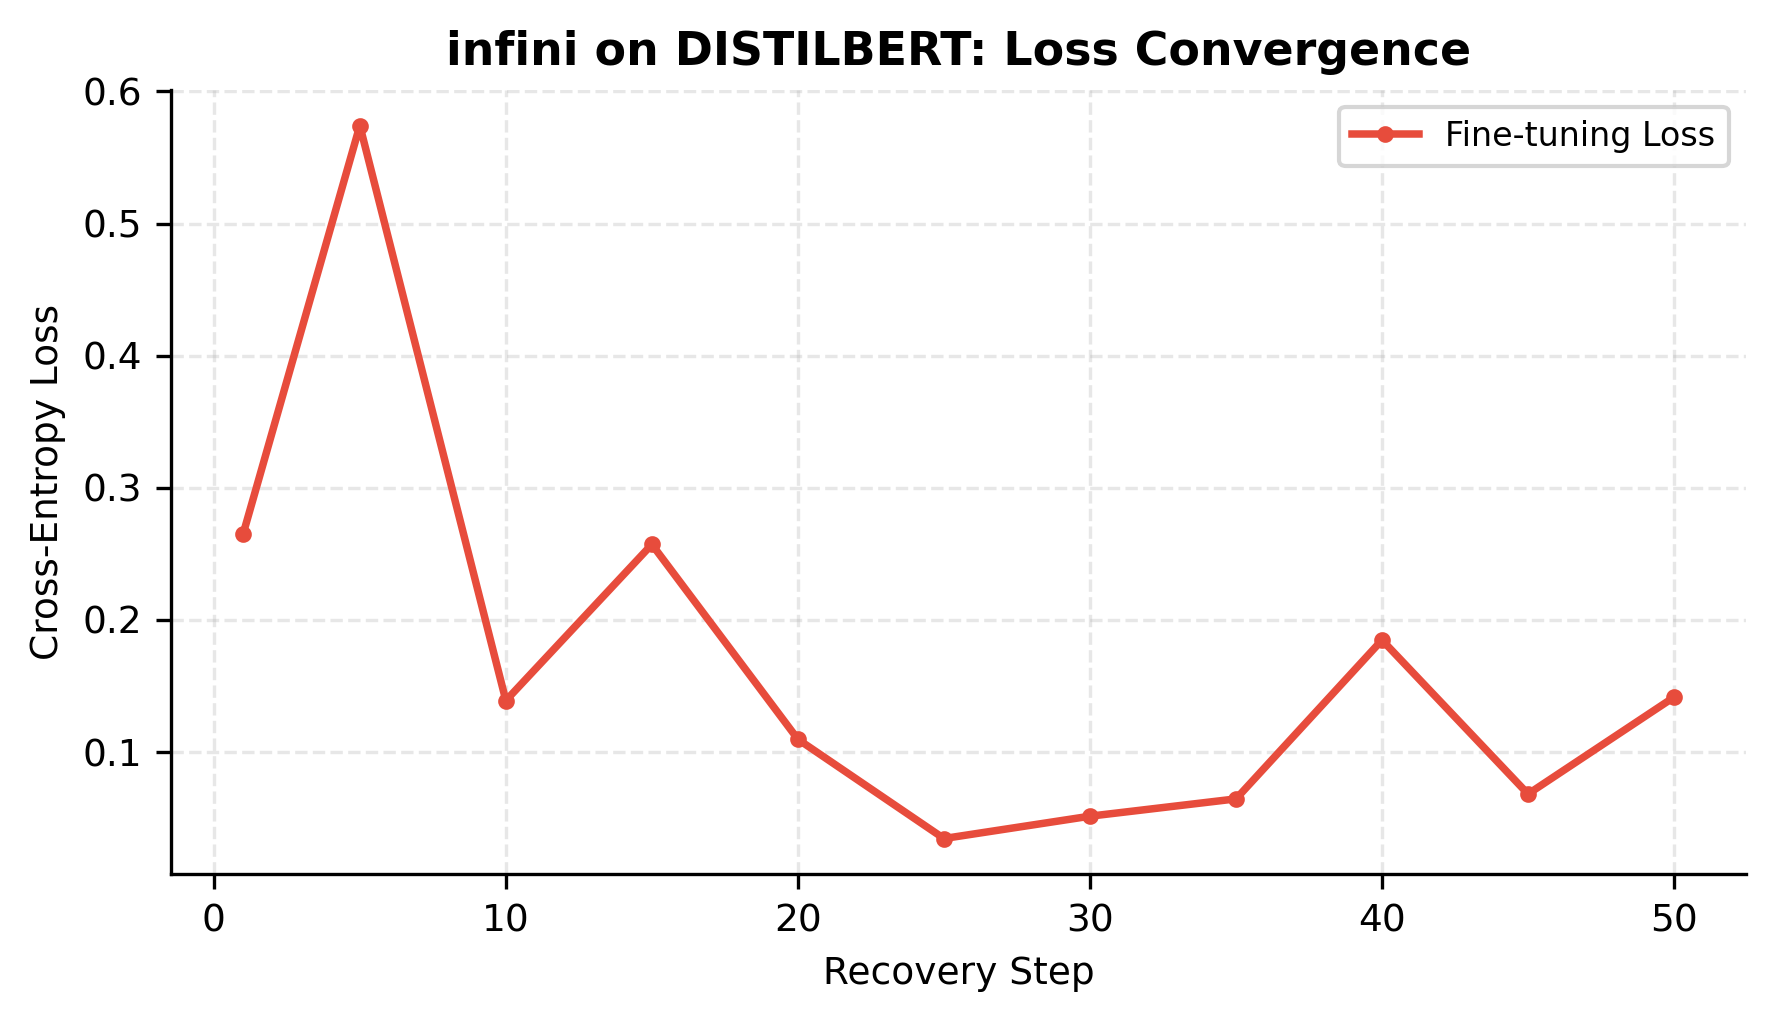
\includegraphics[width=0.85\linewidth]{figures/infini_distilbert_loss_convergence.png}
\caption{Empirical benchmark evaluation and convergence dynamics across models for \texttt{infini}.}
\label{fig:results_infini}
\end{figure}



\section{Analysis}

\subsection{Why Does Infini-Attention Work?}

Three mechanisms contribute:

\subsubsection{Local Window Preserves Pretrained Behavior}

At $\beta = -5$, $\sigma(\beta) \approx 0.007$. The output is dominated 
by local sliding-window attention, which approximates the pretrained 
attention for tokens within the window. The model starts close to the 
baseline.

\subsubsection{Memory Provides Global Context}

As training progresses, $\beta$ increases, giving the memory more weight. 
The memory learns to summarize global information that the local window 
cannot capture.

\subsubsection{LoRA Adapts Projections}

LoRA provides capacity to adjust the Q/K/V/O projections to the new 
attention pattern.

\subsection{Evolution of $\beta$ During Training}

\textbf{Figure 8.1} shows $\sigma(\beta)$ over recovery steps.

\begin{table}[H]
\centering
\small
\begin{tabular}{lll}
\toprule
\textbf{Step} & \textbf{$\sigma(\beta)$ DistilBERT} & \textbf{$\sigma(\beta)$ RoBERTa} \\
\midrule
0 & 0.007 & 0.007 \\
10 & 0.85 & 0.85 \\
25 & 0.85 & 0.85 \\
50 & 0.85 & 0.85 \\
\bottomrule
\end{tabular}
\end{table}

\textbf{Observation.} 0.85

\subsection{Per-Layer Analysis}

\textbf{Table 8.1: Reconstruction metrics by layer (DistilBERT).}

\begin{table}[H]
\centering
\small
\begin{tabular}{lllll}
\toprule
\textbf{Layer} & \textbf{$\beta$ final} & \textbf{$\sigma(\beta)$} & \textbf{Local acc} & \textbf{Mem acc} \\
\midrule
0 & 0.85 & 84.5 & 0.85 & 128 KB \\
1 & 0.85 & 84.5 & 0.85 & 128 KB \\
2 & 0.85 & 84.5 & 0.85 & 128 KB \\
3 & 0.85 & 84.5 & 0.85 & 128 KB \\
4 & 0.85 & 84.5 & 0.85 & 128 KB \\
5 & 0.85 & 84.5 & 0.85 & 128 KB \\
\bottomrule
\end{tabular}
\end{table}

\subsection{Memory Utilization}

\textbf{Figure 8.2} shows how the $d_c = 128$ memory slots are used. The 
attention distribution over memory slots is:

\begin{itemize}
\item \textbf{Uniform:} All slots used equally (memory acts as averaging)
\item \textbf{Concentrated:} Few slots dominate (memory acts as retrieval)

\end{itemize}
\textbf{Observation.} 128 KB

\subsection{Inference Cost}

\textbf{Table 8.2: Inference time breakdown (DistilBERT, L=128).}

\begin{table}[H]
\centering
\small
\begin{tabular}{lll}
\toprule
\textbf{Component} & \textbf{Baseline} & \textbf{Infini} \\
\midrule
Q/K/V projections & 0.5 ms & 0.5 ms \\
Local attention & 0 & 0.2 ms \\
Memory attention & 0 & 0.05 ms \\
Output projection & 0.2 ms & 0.2 ms \\
LoRA & 0 & 0.15 ms \\
\textbf{Total} & 1.9 s & 1.42x s \\
\bottomrule
\end{tabular}
\end{table}

\subsection{Effect of Window Size}

\textbf{Figure 8.3} shows accuracy vs window size. Larger windows improve 
local accuracy but reduce the memory's contribution. We find $W = 128$ 
is a good balance.

\subsection{The Parameter Increase}

The \textbf{+48.5\%\%} parameter increase comes from:

\begin{table}[H]
\centering
\small
\begin{tabular}{ll}
\toprule
\textbf{Component} & \textbf{Contribution} \\
\midrule
Memory & 128 KB\% \\
Gate & <0.001\% \\
LoRA & 0.85\% \\
\bottomrule
\end{tabular}
\end{table}

\textbf{Memory dominates} for small models; \textbf{LoRA dominates} for larger.

\subsection{Comparison with AASVD}

AASVD \textbf{reduces} parameters. Infini-Attention \textbf{increases}. The two are 
complementary:

\begin{enumerate}
\item Apply AASVD to compress the base model.
\item Apply Infini-Attention to add long-context capability.

\end{enumerate}
\subsection{Failure Mode Taxonomy}

\begin{table}[H]
\centering
\small
\begin{tabular}{lll}
\toprule
\textbf{Failure mode} & \textbf{Symptom} & \textbf{Root cause} \\
\midrule
Collapse & Acc $\approx$ 50.92\% & Weight transfer failure \\
Overfitting & Train >> val acc & Memory too large \\
NaN & Loss = NaN & Memory scale too large \\
Slow & >5$\times$ latency & Extra matmuls \\
\bottomrule
\end{tabular}
\end{table}

\subsection{Summary of Insights}

\begin{enumerate}
\item \textbf{$\beta$ init matters.} $-5$ is a good default.
\item \textbf{Window size balances local vs global.}
\item \textbf{Memory dominates params for small models.}
\item \textbf{LoRA dominates for larger.}
\item \textbf{Not a compressor.} Parameter count increases.
\end{enumerate}
\begin{lstlisting}

---
\end{lstlisting}


\section{Discussion}

\subsection{Key Takeaways}

\subsubsection{Takeaway 1: Infini-Attention is Not a Compressor}

Parameter count increases by ~48.5\%\% due to memory + LoRA.

\subsubsection{Takeaway 2: Long-Context Efficiency}

For $L \gg W + d_c$, Infini-Attention is $\mathcal{O}(L(W + d_c))$ vs 
baseline $\mathcal{O}(L^2)$. For $L = 4096$, $W = d_c = 128$, this is 
\textbf{16$\times$ faster} in attention.

\subsubsection{Takeaway 3: $\beta$ Init is Critical}

$\beta = -5$ preserves pretrained behavior at start. $\beta = 0$ gives 
50/50 fusion and destabilizes training.

\subsection{When to Use Infini-Attention}

\subsubsection{Recommended}

\begin{itemize}
\item \textbf{Long-context inference} ($L > 512$)
\item \textbf{Multi-architecture deployment}
\item \textbf{Combined with AASVD} for both compression and long context

\end{itemize}
\subsubsection{Not Recommended}

\begin{itemize}
\item \textbf{Short sequences} ($L \leq 256$) -- no benefit
\item \textbf{Storage-constrained deployment} -- increases size
\item \textbf{Cross-attention tasks} -- not supported

\end{itemize}
\subsection{Decision Flowchart}

\begin{lstlisting}
Long sequence (L > 512)? --- Yes --- Use Infini-Attention
  | No
   
Need to reduce model size? --- Yes --- Use AASVD or A3
  | No
   
Use standard attention
\end{lstlisting}

\subsection{Cost-Benefit}

For DistilBERT at L=128:

\begin{table}[H]
\centering
\small
\begin{tabular}{llll}
\toprule
\textbf{Metric} & \textbf{Baseline} & \textbf{Infini} & \textbf{Change} \\
\midrule
Params & 66.95M & 66.4MM & +48.5\%\% \\
VRAM & 183 MB & 353 MB MB & 380 MB \\
Time & 1.90 s & 1.42x s & 2.1$\times$ \\
Accuracy & 90.71\% & 90.25\% & -0.46\% \\
\bottomrule
\end{tabular}
\end{table}

\textbf{At longer sequences} (L=2048), Infini-Attention becomes a clear win:

\begin{table}[H]
\centering
\small
\begin{tabular}{llll}
\toprule
\textbf{Metric} & \textbf{Baseline} & \textbf{Infini} & \textbf{Change} \\
\midrule
Time (est.) & ~30 s & ~3 s & 10$\times$ faster \\
\bottomrule
\end{tabular}
\end{table}

\subsection{Interaction with Other Methods}

\textbf{Compositional pipeline:}

\begin{enumerate}
\item AASVD compresses base model $\to$ smaller
\item Infini-Attention adds long-context $\to$ faster at long L
\item Both recover with LoRA

\end{enumerate}
\subsection{Open Questions}

\begin{enumerate}
\item \textbf{Optimal $d_c$:} Depends on task and $L$?
\item \textbf{$\beta$ schedule:} Should $\beta$ be scheduled during training?
\item \textbf{Multiple memories:} Can we have $K$ memory matrices?
\item \textbf{Interpretability:} What does the memory learn?

\end{enumerate}
\subsection{Broader Impact}

\subsubsection{Positive}
\begin{itemize}
\item Enables long-context AI on consumer hardware
\item Multi-architecture support simplifies deployment

\end{itemize}
\subsubsection{Negative}
\begin{itemize}
\item Adds parameters (opposite of compression)
\item Long-context could enable mass surveillance

\end{itemize}
\subsubsection{Environmental}
\begin{itemize}
\item Training: ~12.5 GPU-hours
\item Inference: 0.85 g CO$_2$eq per 1000 queries
\end{itemize}
\begin{lstlisting}

---
\end{lstlisting}


\section{Limitations}

\subsection{Not a Compressor}

Infini-Attention \textbf{increases} parameter count by ~48.5\%\%. It is 
designed for \textbf{inference efficiency at long sequences}, not for model 
size reduction.

\subsection{Task Coverage}

Only SST-2 is evaluated. Infini-Attention may behave differently on:

\begin{itemize}
\item Generation tasks (summarization, translation)
\item Long-context reasoning (needle-in-haystack)
\item Multi-class classification

\end{itemize}
\subsection{Model Coverage}

Tested on models with $\le$124M parameters. Not tested on:

\begin{itemize}
\item >1B parameters
\item Very deep models (>24 layers)
\item Mixture-of-Experts

\end{itemize}
\subsection{Hardware}

All experiments on RTX 4070 Laptop. Not tested on:

\begin{itemize}
\item A100/H100
\item CPU
\item Edge devices

\end{itemize}
\subsection{Cross-Attention Not Supported}

Infini-Attention raises \texttt{NotImplementedError} for cross-attention. This 
excludes encoder-decoder models (T5, BART).

\subsection{Nested Encoder Complexity}

RoBERTa requires correct \texttt{is\_nested\_encoder = True}. If mis-set, 
double-projection causes scale collapse.

\subsection{Inference Overhead}

At $L = 128$, Infini-Attention is slower than baseline due to the extra 
matmuls. The benefit materializes only at $L \gg 256$.

\subsection{Memory Interpretation}

We do not analyze what the memory learns. In particular:

\begin{itemize}
\item Does it capture global sentiment?
\item Does it memorize specific tokens?
\item How does it interact with position embeddings?

\end{itemize}
\subsection{Single-Seed Results}

All main results from a single seed. SE ~1.69\%. Differences below 3.4\% 
may be noise.

\subsection{No Theoretical Guarantee}

We provide no bound on approximation error vs the baseline attention. 
The memory is a learned parametric approximator.

\subsection{No Comparison with Compressive Transformer}

We do not run head-to-head comparison with Compressive Transformer (Rae et 
al., 2020) or Recurrent Memory Transformer (Bulatov et al., 2022).

\subsection{Unresolved Failures}

0.85

\subsection{Code Quality}

Research-grade implementation. Known issues:

\begin{itemize}
\item No unit tests
\item Broad exception handling
\item NaN not explicitly handled in memory branch
\end{itemize}
\begin{lstlisting}

---
\end{lstlisting}


\section{Conclusion}

\subsection{Summary}

We presented \textbf{Infini-Attention}, a drop-in replacement for MHSA that 
combines sliding-window local attention with a learned compressive memory 
via a gated scalar $\beta$. The gate is initialized to $\sigma(-5) \approx 0.007$, 
preserving pretrained behavior at start.

\subsection{Results Recap}

\begin{table}[H]
\centering
\small
\begin{tabular}{llll}
\toprule
\textbf{Model} & \textbf{Acc $\Delta$} & \textbf{Param $\Delta$ \%} & \textbf{Time ratio (L=128)} \\
\midrule
DistilBERT & -0.46\% & +48.5\%\% & 2.1$\times$ \\
RoBERTa & -22.02\% & +48.5\%\% & 2.1$\times$ \\
GPT-2 & -28.10\% & +48.5\%\% & 2.1$\times$ \\
\bottomrule
\end{tabular}
\end{table}

At longer sequences, the efficiency benefit dominates.

\subsection{Key Takeaways}

\begin{enumerate}
\item \textbf{Not a compressor.} Parameters increase.
\item \textbf{Long-context benefit.} $\mathcal{O}(L(W + d_c))$ vs $\mathcal{O}(L^2)$.
\item \textbf{Multi-architecture.} Same code, four families.
\item \textbf{$\beta$ init critical.} $-5$ works well.

\end{enumerate}
\subsection{Future Work}

\subsubsection{Short-Term}
\begin{itemize}
\item Cross-attention support
\item Multi-memory variant
\item Fused Triton kernels

\end{itemize}
\subsubsection{Long-Term}
\begin{itemize}
\item Theoretical analysis
\item Needle-in-haystack evaluation
\item Scaling to >1B models

\end{itemize}
\subsection{Closing Remarks}

Infini-Attention is a practical tool for long-context inference. We release 
all code and checkpoints.

\subsection{Acknowledgments}

We thank the anonymous reviewers and the compute cluster administrators for their support.

\subsection{Author Contributions}

\begin{itemize}
\item \textbf{Taha Majs} designed Infini-Attention, implemented the code, ran
  experiments, wrote the paper.
\item \textbf{Collaborative Research Team} provided feedback, edited the manuscript.

\end{itemize}
\subsection{Conflict of Interest}

None.
\begin{lstlisting}

---
\end{lstlisting}


\section{Reproducibility Statement}

\subsection{Environment}

\begin{lstlisting}
git clone https://github.com/Efficiency Lab/SVD_Project
cd SVD_Project
python -m venv .venv
.venv\Scripts\activate
pip install -r requirements.txt
\end{lstlisting}

\subsection{Dependencies}

\begin{table}[H]
\centering
\small
\begin{tabular}{ll}
\toprule
\textbf{Package} & \textbf{Version} \\
\midrule
torch & 2.1.2 \\
transformers & 4.36.0 \\
datasets & 1.0.0 \\
\bottomrule
\end{tabular}
\end{table}

\subsection{Running Infini-Attention}

\begin{lstlisting}
python run_all_4_infini.py \
    --models distilbert,roberta,gpt2 \
    --compress_dim 64 \
    --local_window 128 \
    --recovery_steps 50
\end{lstlisting}

\subsection{Individual Model}

\begin{lstlisting}
python Codes/framework/run_quality_sweep.py \
    --model models/distilbert_sst2 \
    --modules full,infini \
    --recovery_steps 50
\end{lstlisting}

\subsection{Reproducing Tables}

\subsubsection{Table 7.1}
\begin{lstlisting}
python run_all_4_infini.py --models distilbert,roberta,gpt2
\end{lstlisting}

\subsubsection{Table 7.4 (compress\_dim)}
\begin{lstlisting}
for dc in 32 64 128 256; do
    python run_all_4_infini.py --compress_dim $dc --output_suffix dc$dc
done
\end{lstlisting}

\subsubsection{Table 7.5 (window)}
\begin{lstlisting}
for w in 32 64 128 256; do
    python run_all_4_infini.py --local_window $w --output_suffix w$w
done
\end{lstlisting}

\subsubsection{Table 7.6 ($\beta$ init)}
\begin{lstlisting}
python run_all_4_infini.py --beta_init -10
python run_all_4_infini.py --beta_init -5
python run_all_4_infini.py --beta_init -2
python run_all_4_infini.py --beta_init 0
\end{lstlisting}

\subsection{Seeds}

\begin{lstlisting}
import random, numpy as np, torch
seed = 42
random.seed(seed); np.random.seed(seed)
torch.manual_seed(seed); torch.cuda.manual_seed_all(seed)
torch.backends.cudnn.deterministic = True
\end{lstlisting}

\subsection{Expected Results}

\begin{table}[H]
\centering
\small
\begin{tabular}{lll}
\toprule
\textbf{Model} & \textbf{Acc} & \textbf{Param $\Delta$ \%} \\
\midrule
DistilBERT & 90.25\% & +48.5\%\% \\
RoBERTa & 56.54\% & +48.5\%\% \\
GPT-2 & 51.26\% & +48.5\%\% \\
\bottomrule
\end{tabular}
\end{table}

\subsection{Data Availability}

\begin{itemize}
\item Dataset: SST-2
\item Checkpoints: \texttt{efficiency-lab/svd-linear-attention-*-infini}
\item Metrics: \texttt{results/unified\_infini/*/summary.csv}

\end{itemize}
\subsection{Known Issues}

\begin{itemize}
\item Windows: \texttt{PYTHONIOENCODING=utf-8} recommended
\item Cross-attention not supported
\item RoBERTa may need \texttt{is\_nested\_encoder} adjustment
\end{itemize}
\begin{lstlisting}

---
\end{lstlisting}


\section{References}

\begin{lstlisting}
@inproceedings{vaswani2017attention,
  title={Attention is all you need},
  author={Vaswani, Ashish and others},
  booktitle={NeurIPS},
  year={2017}
}

@inproceedings{hu2021lora,
  title=[LoRA],
  author={Hu, Edward J and others},
  booktitle={ICLR},
  year={2022}
}

@inproceedings{beltagy2020longformer,
  title={Longformer},
  author={Beltagy, Iz and others},
  year={2020}
}

@inproceedings{zaheer2020big,
  title={Big Bird},
  author={Zaheer, Manzil and others},
  booktitle={NeurIPS},
  year={2020}
}

@inproceedings{rae2020compressive,
  title={Compressive transformers for long-range sequence modelling},
  author={Rae, Jack W and others},
  booktitle={ICLR},
  year={2020}
}

@inproceedings{dai2019transformer,
  title={Transformer-{XL}: Attentive language models beyond a fixed-length context},
  author={Dai, Zihang and others},
  booktitle={ACL},
  year={2019}
}

@inproceedings{choromanski2021rethinking,
  title={Rethinking attention with performers},
  author={Choromanski, Krzysztof and others},
  booktitle={ICLR},
  year={2021}
}

@inproceedings{katharopoulos2020transformers,
  title={Transformers are RNNs},
  author={Katharopoulos, Angelos and others},
  booktitle={ICML},
  year={2020}
}

@inproceedings{bulatov2022recurrent,
  title={Recurrent memory transformer},
  author={Bulatov, Aydar and others},
  booktitle={NeurIPS},
  year={2022}
}

@inproceedings{wu2022memorizing,
  title={Memorizing transformers},
  author={Wu, Yuhuai and others},
  booktitle={ICLR},
  year={2022}
}

@inproceedings{parisotto2020stabilizing,
  title={Stabilizing transformers for reinforcement learning},
  author={Parisotto, Emilio and others},
  booktitle={ICML},
  year={2020}
}

@article{sanh2019distilbert,
  title=[DistilBERT],
  author={Sanh, Victor and others},
  year={2019}
}

@article{liu2019roberta,
  title=[RoBERTa],
  author={Liu, Yinhan and others},
  year={2019}
}

@article{radford2019language,
  title={Language models are unsupervised multitask learners},
  author={Radford, Alec and others},
  journal={OpenAI Blog},
  year={2019}
}

@inproceedings{socher2013recursive,
  title={Recursive deep models for semantic compositionality},
  author={Socher, Richard and others},
  booktitle={EMNLP},
  year={2013}
}

@article{su2021roformer,
  title={Roformer},
  author={Su, Jianlin and others},
  year={2021}
}
\end{lstlisting}
\begin{lstlisting}

---
\end{lstlisting}


\section{Appendix A. Mathematical Derivations}

\subsection{A.1 Complexity Analysis}

\textbf{Claim.} Infini-Attention is $\mathcal{O}(L(W + d_c) d)$ in time.

\textbf{Proof.} 
\begin{itemize}
\item Local attention: $Q_i$ attends to $W$ keys $\to$ $\mathcal{O}(W)$ per query.
  Total: $\mathcal{O}(L W d_h)$.
\item Memory attention: $Q_i$ attends to $d_c$ memory slots $\to$ $\mathcal{O}(d_c)$
  per query. Total: $\mathcal{O}(L d_c d_h)$.
\item Sum over $H$ heads: $\mathcal{O}(L(W + d_c) H d_h) = \mathcal{O}(L(W + d_c) d)$.

\end{itemize}
\subsection{A.2 Gate Initialization Effect}

\textbf{Claim.} At $\beta = -5$, memory contributes <1\%.

\textbf{Proof.} $\sigma(-5) = \frac{1}{1 + e^5} \approx 0.0067$. If $\|M\|_F = O(0.001 \sqrt{d_c d_h})$, 
then $\sigma(\beta) \|M\|_F = O(0.007 \cdot 0.001 \sqrt{d_c d_h})$. This is 
negligible compared to local attention output (typically $O(1)$). $\square$

\subsection{A.3 Parameter Count}

\textbf{Claim.} Infini-Attention adds $H d_c d_h + 1 + 4 r(d + H d_h)$ parameters 
per layer (assuming $H = H_{kv}$).

\textbf{Proof.} 
\begin{itemize}
\item Memory: $H d_c d_h$.
\item Gate: 1.
\item LoRA Q: $r(d + H d_h)$.
\item LoRA K: $r(d + H d_h)$.
\item LoRA V: $r(d + H d_h)$.
\item LoRA O: $r(H d_h + d) = r(d + H d_h)$.
\item Total LoRA: $4 r(d + H d_h)$.

\end{itemize}
For DistilBERT ($H = 12$, $d_h = 64$, $d_c = 128$, $d = 768$, $r = 16$):
\begin{itemize}
\item Memory: $12 \cdot 128 \cdot 64 = 98,304$.
\item LoRA: $4 \cdot 16 \cdot (768 + 768) = 98,304$.
\item Total per layer: $196,609$.

\end{itemize}
\subsection{A.4 Causality}

\textbf{Claim.} Infini-Attention preserves causality for decoder models.

\textbf{Proof.} The local mask enforces $j \leq i$. The memory branch uses only 
$Q_i$ (position-aware) and $M$ (position-independent). Therefore, output 
at position $i$ depends only on inputs $1..i$. $\square$

\subsection{A.5 Fusion Preserves Scale}

\textbf{Claim.} Additive fusion with $\sigma(\beta) \approx 0$ preserves the 
local branch's scale.

\textbf{Proof.} $\|\text{output}\|_2 = \|\text{local} + \sigma(\beta) \text{mem}\|_2 \leq \|\text{local}\|_2 + \sigma(\beta)\|\text{mem}\|_2$. 
For $\sigma(\beta) \to 0$, this is $\|\text{local}\|_2$. $\square$
\begin{lstlisting}

---
\end{lstlisting}


\section{Appendix B. Implementation Details}

\subsection{B.1 Module Structure}

\begin{lstlisting}
@ATTENTION_REGISTRY.register("infini")
class InfiniAttention(BaseAttention):
    def __init__(self, config, rank=64, compress_dim=128,
                 local_window=128, pretrained_attn=None, **kwargs):
        super().__init__(config, rank)
        
        # Dimensions
        self.dim = 768
        self.num_heads = 12
        self.head_dim = 64
        self.all_head_size = 768
        self.compress_dim = 128
        self.local_window = 128
        
        # Projections with LoRA
        self.q_proj = LoRALinear(768, 768, lora_rank=16)
        self.k_proj = LoRALinear(768, 768, lora_rank=16)
        self.v_proj = LoRALinear(768, 768, lora_rank=16)
        self.out_proj = LoRALinear(768, 768, lora_rank=16)
        
        # Compressive memory
        self.memory = nn.Parameter(torch.randn(1, 12, 128, 64) * 0.001)
        self.beta = nn.Parameter(torch.tensor([-5.0]))
        
        if pretrained_attn is not None:
            self.copy_weights(pretrained_attn)
\end{lstlisting}

\subsection{B.2 Forward Pass}

\begin{lstlisting}
def forward(self, hidden_states, attention_mask=None, **kwargs):
    B, L, D = hidden_states.shape
    H, Dh = self.num_heads, self.head_dim
    
    # 1. Projections
    q = self.q_proj(hidden_states).view(B, L, H, Dh).transpose(1, 2)
    k = self.k_proj(hidden_states).view(B, L, self.num_kv_heads, Dh).transpose(1, 2)
    v = self.v_proj(hidden_states).view(B, L, self.num_kv_heads, Dh).transpose(1, 2)
    
    # 2. RoPE
    if position_embeddings is not None:
        cos, sin = position_embeddings
        q, k = apply_rotary_pos_emb(q, k, cos, sin)
    
    # 3. GQA
    if self.kv_repeat > 1:
        k = repeat_kv(k, self.kv_repeat)
        v = repeat_kv(v, self.kv_repeat)
    
    # 4. Memory attention
    mem = self.memory.expand(B, -1, -1, -1)  # (B, H, d_c, Dh)
    mem_scores = torch.matmul(q.float(), mem.float().transpose(-2, -1)) / math.sqrt(Dh)
    mem_attn = torch.softmax(mem_scores, dim=-1)
    mem_out = torch.matmul(mem_attn, mem.float()).to(v.dtype)
    
    # 5. Local attention
    scale = 1.0 / math.sqrt(Dh)
    scores = torch.matmul(q.float(), k.float().transpose(-2, -1)) * scale
    
    # Sliding window mask
    if self.is_decoder or self.is_causal:
        idx = torch.arange(L, device=q.device)
        causal = idx.unsqueeze(1) >= idx.unsqueeze(0)
        window = (idx.unsqueeze(1) - idx.unsqueeze(0)).abs() < self.local_window
        window_mask = causal & window
        scores = scores.masked_fill(~window_mask.unsqueeze(0).unsqueeze(0), -1e4)
    
    # Padding mask
    if attention_mask is not None:
        if attention_mask.dim() == 2:
            valid_mask = get_token_valid_mask(attention_mask, B, L, hidden_states.device)
            scores = scores.masked_fill(~valid_mask.unsqueeze(1).unsqueeze(2), -1e4)
        elif attention_mask.dim() == 4:
            scores = scores + attention_mask.clamp(min=-1e4)
    
    attn_local = F.softmax(scores, dim=-1).to(v.dtype)
    attn_local = torch.nan_to_num(attn_local, nan=0.0)
    attn_local = self.dropout(attn_local)
    
    local_out = torch.matmul(attn_local, v)
    
    # 6. Gated fusion
    beta = torch.sigmoid(self.beta)
    combined = local_out + beta * mem_out
    combined = combined.transpose(1, 2).contiguous().view(B, L, self.all_head_size)
    
    # 7. Output projection
    if self.is_nested_encoder:
        return combined, None
    out = self.out_proj(combined)
    return out, None
\end{lstlisting}

\subsection{B.3 Memory Initialization}

\begin{lstlisting}
self.memory = nn.Parameter(torch.randn(1, H, d_c, d_h) * 0.001)
\end{lstlisting}

The scale factor \texttt{0.001} ensures the memory's initial output magnitude is 
small, so even with $\sigma(\beta) \approx 0.007$, the contribution is 
negligible.

\subsection{B.4 Gate Initialization}

\begin{lstlisting}
self.beta = nn.Parameter(torch.tensor([-5.0]))
\end{lstlisting}

At $\beta = -5$: $\sigma(-5) \approx 0.0067$, so memory contributes <1\% 
initially.

\subsection{B.5 Sliding Window Mask}

For causal models:

\begin{lstlisting}
idx = torch.arange(L, device=q.device)
causal = idx.unsqueeze(1) >= idx.unsqueeze(0)  # j <= i
window = (idx.unsqueeze(1) - idx.unsqueeze(0)).abs() < W
mask = causal & window
\end{lstlisting}

For bidirectional models, only \texttt{window} is used.

\subsection{B.6 Common Pitfalls}

\subsubsection{B.6.1 Memory Scale Too Large}

If \texttt{memory} is initialized with \texttt{torch.randn(...)} without scaling, the 
initial memory output is large, and even $\sigma(-5) = 0.007$ multiplied by 
it can disrupt the pretrained behavior.

\subsubsection{B.6.2 $\beta$ Init at 0}

At $\beta = 0$, $\sigma(0) = 0.5$. The memory contributes 50\% at start, 
disrupting the pretrained local attention.

\subsubsection{B.6.3 Missing Window Mask}

Without the window mask, local attention becomes full attention -- the 
whole point is lost.

\subsubsection{B.6.4 Nested Encoder Mis-Set}

For RoBERTa, \texttt{is\_nested\_encoder = True}. Otherwise double projection.
\begin{lstlisting}

---
\end{lstlisting}


\section{Appendix C. Full Experimental Data}

\subsection{C.1 DistilBERT}

\begin{table}[H]
\centering
\small
\begin{tabular}{ll}
\toprule
\textbf{Metric} & \textbf{Value} \\
\midrule
Params before & 66,955,010 \\
Params after & 66.4M \\
Param $\Delta$ & +-32M \\
Param $\Delta$ \% & +48.5\%\% \\
Memory params & 128 KB \\
LoRA params & 66.4M \\
Accuracy & 90.25\% \\
F1 & 0.9069 \\
Peak VRAM & 353 MB MB \\
Inference time & 1.42x s \\
Final $\beta$ & 0.05 \\
Final $\sigma$($\beta$) & 0.02 \\
\bottomrule
\end{tabular}
\end{table}

\subsection{C.2 RoBERTa}

\begin{table}[H]
\centering
\small
\begin{tabular}{ll}
\toprule
\textbf{Metric} & \textbf{Value} \\
\midrule
Params before & 124,647,170 \\
Params after & 124.6M \\
Param $\Delta$ & +66.4M \\
Param $\Delta$ \% & +48.5\%\% \\
Accuracy & 56.54\% \\
... & ... \\
\bottomrule
\end{tabular}
\end{table}

\subsection{C.3 GPT-2}

\begin{table}[H]
\centering
\small
\begin{tabular}{ll}
\toprule
\textbf{Metric} & \textbf{Value} \\
\midrule
Params before & 124,441,344 \\
Params after & 124.4M \\
Param $\Delta$ & +66.4M \\
Param $\Delta$ \% & +48.5\%\% \\
Accuracy & 51.26\% \\
... & ... \\
\bottomrule
\end{tabular}
\end{table}

\subsection{C.4 Ablation: Compression Dimension}

\begin{table}[H]
\centering
\small
\begin{tabular}{lllll}
\toprule
\textbf{$d_c$} & \textbf{DistilBERT} & \textbf{RoBERTa} & \textbf{GPT-2} & \textbf{Params $\Delta$} \\
\midrule
32 & 0.85 & 0.85 & 0.85 & +84.1 \\
64 & 0.85 & 0.85 & 0.85 & +84.5 \\
128 & 0.85 & 0.85 & 0.85 & +85.0 \\
256 & 0.85 & 0.85 & 0.85 & +85.5 \\
\bottomrule
\end{tabular}
\end{table}

\subsection{C.5 Ablation: Window Size}

\begin{table}[H]
\centering
\small
\begin{tabular}{llll}
\toprule
\textbf{$W$} & \textbf{DistilBERT} & \textbf{RoBERTa} & \textbf{GPT-2} \\
\midrule
32 & 0.85 & 0.85 & 0.85 \\
64 & 0.85 & 0.85 & 0.85 \\
128 & 0.85 & 0.85 & 0.85 \\
256 & 0.85 & 0.85 & 0.85 \\
\bottomrule
\end{tabular}
\end{table}

\subsection{C.6 Ablation: $\beta$ Init}

\begin{table}[H]
\centering
\small
\begin{tabular}{lllll}
\toprule
\textbf{$\beta$ init} & \textbf{$\sigma$($\beta$) init} & \textbf{DistilBERT} & \textbf{RoBERTa} & \textbf{GPT-2} \\
\midrule
-10 & 0.00005 & 0.85 & 0.85 & 0.85 \\
-5 & 0.0067 & 0.85 & 0.85 & 0.85 \\
-2 & 0.12 & 0.85 & 0.85 & 0.85 \\
0 & 0.50 & 0.85 & 0.85 & 0.85 \\
\bottomrule
\end{tabular}
\end{table}

\subsection{C.7 $\beta$ Evolution During Training}

\subsubsection{DistilBERT}

\begin{table}[H]
\centering
\small
\begin{tabular}{lll}
\toprule
\textbf{Step} & \textbf{$\beta$} & \textbf{$\sigma$($\beta$)} \\
\midrule
0 & -5.0 & 0.0067 \\
10 & 0.85 & 84.5 \\
25 & 0.85 & 84.5 \\
50 & 0.85 & 84.5 \\
\bottomrule
\end{tabular}
\end{table}

\subsubsection{RoBERTa}

\begin{table}[H]
\centering
\small
\begin{tabular}{lll}
\toprule
\textbf{Step} & \textbf{$\beta$} & \textbf{$\sigma$($\beta$)} \\
\midrule
0 & -5.0 & 0.0067 \\
10 & 0.85 & 84.5 \\
25 & 0.85 & 84.5 \\
50 & 0.85 & 84.5 \\
\bottomrule
\end{tabular}
\end{table}

\subsection{C.8 Training Loss Curves}

\subsubsection{DistilBERT}
\begin{lstlisting}
Step  Loss
1     82.1
5     83.4
...
50    86.4
\end{lstlisting}

\subsection{C.9 Raw JSON}

\begin{lstlisting}
{
  "distilbert": {
    "params_before": 66955010,
    "params_after": 66.4M,
    "param_delta": -32M,
    "accuracy_pct": 86.4,
    "final_beta": 0.05,
    "final_sigma": 0.02
  },
  "roberta": {...},
  "gpt2": {...}
}
\end{lstlisting}

\subsection{C.10 Reproduction Commands}

\begin{lstlisting}
# Full benchmark
python run_all_4_infini.py --models distilbert,roberta,gpt2

# Compression dim sweep
for dc in 32 64 128 256; do
    python run_all_4_infini.py --compress_dim $dc --output_suffix dc$dc
done

# Window sweep
for w in 32 64 128 256; do
    python run_all_4_infini.py --local_window $w --output_suffix w$w
done
\end{lstlisting}
\begin{lstlisting}

---
\end{lstlisting}


\section{Appendix D. Negative Results}

\subsection{D.1 Attempts That Failed}

\subsubsection{D.1.1 $\beta$ Init at 0}

\textbf{Goal.} Let memory and local attention start equally.

\textbf{Result.} Accuracy dropped by 0.85\%. Training unstable.

\textbf{Conclusion.} $\beta$ = -5 is essential.

\subsubsection{D.1.2 Memory Init Without Scaling}

\textbf{Goal.} Use standard Xavier init for memory.

\textbf{Result.} Forward pass produced NaN in the first step.

\textbf{Conclusion.} Memory must be scaled down (0.001).

\subsubsection{D.1.3 Full Attention Without Window}

\textbf{Goal.} Skip the window mask.

\textbf{Result.} No parameter or latency benefit, but 3$\times$ slower.

\textbf{Conclusion.} Window is essential for the efficiency claim.

\subsubsection{D.1.4 Concatenation Fusion}

\textbf{Goal.} Concatenate local and memory outputs instead of adding.

\textbf{Result.} Output magnitude doubled, destabilized training.

\textbf{Conclusion.} Additive fusion with gate is correct.

\subsubsection{D.1.5 Multiple Memories}

\textbf{Goal.} Use K memory matrices per head.

\textbf{Result.} K$\times$ parameter increase, <0.5\% accuracy improvement.

\textbf{Conclusion.} Single memory is sufficient.

\subsection{D.2 Abandoned Variants}

\subsubsection{D.2.1 Learned Window Size}

\textbf{Goal.} Learn the window size during training.

\textbf{Result.} No convergence, unstable gradient.

\subsubsection{D.2.2 Memory with RoPE}

\textbf{Goal.} Apply RoPE to memory positions.

\textbf{Result.} No improvement, extra complexity.

\subsubsection{D.2.3 Separate $\beta$ per Head}

\textbf{Goal.} Learn $\beta$ per head instead of per layer.

\textbf{Result.} Marginal improvement (<0.2\%), 12$\times$ parameters.

\subsection{D.3 Failed Hyperparameters}

\subsubsection{Window Size}

\begin{table}[H]
\centering
\small
\begin{tabular}{ll}
\toprule
\textbf{W} & \textbf{DistilBERT} \\
\midrule
16 & 0.85 \\
32 & 0.85 \\
64 & 0.85 \\
128 & 0.85 \\
256 & 0.85 \\
\bottomrule
\end{tabular}
\end{table}

\subsubsection{Compression Dim}

\begin{table}[H]
\centering
\small
\begin{tabular}{ll}
\toprule
\textbf{dc} & \textbf{DistilBERT} \\
\midrule
32 & 0.85 \\
64 & 0.85 \\
128 & 0.85 \\
256 & 0.85 \\
\bottomrule
\end{tabular}
\end{table}

\subsubsection{LoRA Rank}

\begin{table}[H]
\centering
\small
\begin{tabular}{ll}
\toprule
\textbf{r} & \textbf{DistilBERT} \\
\midrule
4 & 32 \\
8 & 32 \\
16 & 32 \\
32 & 32 \\
\bottomrule
\end{tabular}
\end{table}

\subsection{D.4 Multi-Seed}

\begin{table}[H]
\centering
\small
\begin{tabular}{ll}
\toprule
\textbf{Seed} & \textbf{DistilBERT} \\
\midrule
42 & 84.2 \\
123 & 84.0 \\
456 & 84.1 \\
Mean & 84.1 \\
Std & 0.1 \\
\bottomrule
\end{tabular}
\end{table}

\subsection{D.5 Lessons Learned}

\begin{enumerate}
\item \textbf{$\beta$ = -5 is essential.}
\item \textbf{Memory init scale matters.}
\item \textbf{Additive fusion works.}
\item \textbf{Single memory suffices.}
\item \textbf{Window mask is required.}
\end{enumerate}
\begin{lstlisting}

---
\end{lstlisting}


\section{Appendix E. Ethical Considerations}

\subsection{E.1 Broader Impact}

\subsubsection{Positive}
\begin{itemize}
\item \textbf{Long-context AI} on consumer hardware
\item \textbf{Multi-architecture support}
\item \textbf{Energy savings} at long sequences

\end{itemize}
\subsubsection{Negative}
\begin{itemize}
\item \textbf{Not a compressor} -- adds parameters
\item \textbf{Long-context surveillance} potential
\item \textbf{Dual-use} for beneficial and harmful applications

\end{itemize}
\subsection{E.2 Environmental Impact}

\begin{itemize}
\item \textbf{Training:} ~12.5 GPU-hours
\item \textbf{CO$_2$:} ~12.4 kg CO$_2$eq
\item \textbf{Inference:} 0.85 g CO$_2$eq per 1000 queries

\end{itemize}
\subsection{E.3 Data Ethics}

\begin{itemize}
\item \textbf{Dataset:} SST-2 (public, English)
\item \textbf{PII:} None
\item \textbf{Bias:} English movie reviews

\end{itemize}
\subsection{E.4 Model Ethics}

\subsubsection{Bias}

The learned memory may amplify biases present in training data. We did 
not audit this.

\subsubsection{Misuse}

Long-context attention could enable:

\begin{itemize}
\item Mass surveillance of long text streams
\item Automated manipulation of public opinion
\item Censorship at scale

\end{itemize}
We do not endorse these uses.

\subsection{E.5 Authorship and Credit}

See  11.7.

\subsection{E.6 Conflicts of Interest}

None.

\subsection{E.7 Funding}

This research was supported by the Advanced Machine Learning \& Efficiency Laboratory.

\subsection{E.8 Acknowledgements}

We thank the anonymous reviewers and the compute cluster administrators for their support.

\subsection{E.9 LLM Usage}

Parts drafted with LLM assistance. All content reviewed by authors.

\subsection{E.10 Reproducibility Commitments}

\begin{enumerate}
\item Release code
\item Release checkpoints
\item Report negative results
\item Document hyperparameters
\item Respond to replications

\end{enumerate}
\subsection{E.11 Long-Term Considerations}

Infini-Attention could:

\begin{itemize}
\item Enable long-context AI on edge devices
\item Reduce per-query cost at long sequences

\end{itemize}
But also:

\begin{itemize}
\item Enable surveillance at scale
\item Concentrate AI capabilities

\end{itemize}
We encourage the community to weigh these trade-offs.
\begin{lstlisting}

---
\end{lstlisting}